%
% ---------------------------------------------------
%
% Proyecto Final de Carrera: EMIR
% Autor: Pedro Hernández Martín <alu3679@etsii.ull.es>
% Capítulo: Estado del arte
% Fichero: Cap2_estado_del_arte.tex
%
% ----------------------------------------------------
%

\chapter{Tecnologías y herramientas relacionadas} \label{chap:estado}

A continuación se dan a conocer algunas tecnologías o conocimientos que han 
resultado necesarios para el proyecto, o se han planteado como tal.

\section{Parsers XML}

Un analizador sintáctico \cite{Wiki:2013:ANA} (en inglés parser) es una de las 
partes de un compilador que transforma su entrada en un árbol de derivación.
El análisis sintáctico convierte el texto de entrada en otras estructuras 
(comúnmente árboles), que son más útiles para el posterior análisis y capturan 
la jerarquía implícita de la entrada. Un analizador léxico crea tokens de una 
secuencia de caracteres de entrada y son estos tokens los que son procesados 
por el analizador sintáctico para construir la estructura de datos, por ejemplo 
un árbol de análisis o árboles de sintaxis abstracta.

El uso más común de los analizadores sintácticos es como parte de la fase de 
análisis de los compiladores, de modo que tienen que analizar el código fuente 
del lenguaje. Los lenguajes de programación tienden a basarse en gramáticas 
libres de contexto, debido a que se pueden escribir analizadores rápidos y 
eficientes para éstas.

Las gramáticas libres de contexto tienen una expresividad limitada y sólo pueden 
expresar un conjunto limitado de lenguajes. Informalmente la razón de esto es
que la memoria de un lenguaje de este tipo es limitada, la gramática no puede 
recordar la presencia de una construcción en una entrada arbitrariamente larga y
esto es necesario en un lenguaje en el que, por ejemplo, una variable debe ser
declarada antes de que pueda ser referenciada. Las gramáticas más complejas no 
pueden ser analizadas de forma eficiente. Por estas razones es común crear un 
analizador permisivo para una gramática libre de contexto que acepta un
superconjunto del lenguaje (acepta algunas construcciones inválidas); después
del análisis inicial las construcciones incorrectas pueden ser filtradas.

Puesto que la entrada y salida de la aplicación \CSUO{} se encuentran
descritas en XML, se aprovechará unos de los muchos parsers opensource
disponibles en Internet para, por un lado, comprobar que la entrada no tiene
errores, y por otro, transformar estos datos en las estructuras que necesita
nuestra aplicación. Existen muchas librerías que nos facilitan la lectura y
escritura de este tipo de ficheros; como se desea distribuir la aplicación para
que cualquiera la pueda utilizar, es muy recomendable emplear una librería
estándar (o muy popular) que sea eficiente.

\subsection{Xerces-C++}

Xerces-C++ \cite{Web:Xerces} es un analizador de XML válido escrito en un
subconjunto portable de C++. Xerces-C++ hace que sea fácil darle a su aplicación
la capacidad de leer y escribir datos XML. Proporciona una biblioteca compartida
para analizar, generar, manipular y validar documentos XML utilizando DOM, SAX y
APIs de SAX2. Xerces-C++ es fiel a la recomendada XML 1.0 y a muchos estándares
asociados.

El analizador proporciona un alto rendimiento, modularidad y escalabilidad.
Código fuente, muestras y documentación de la API se proporcionan con el
analizador. Para que resulte portable se ha tenido cuidado de hacer un uso
mínimo de las plantillas, no usa RTTI, y un uso mínimo de \texttt{\#ifdefs}. Sin
embargo este analizador se descartó debido a que encontramos otro que se
ajustaba mejor a nuestras necesidades.

\subsection{Mini-XML}

Mini-XML \cite{Web:Mini-XML} es una pequeña librería XML que se utiliza
para leer y escribir XML y archivos de datos estilo XML en nuestra aplicación
sin necesidad de usar grandes librerías no estandarizadas. Mini-XML sólo
requiere de un compilador de C compatible con ANSI (GCC funciona, al igual que 
la mayoría de compiladores ANSI C).

Mini-XML permite la lectura de UTF-8 y UTF-16 y la escritura de UTF-8 en
ficheros XML codificados y cadenas. Los datos se almacenan en una lista enlazada
con estructura de árbol, conservando la jerarquía de datos XML, y los nombres de 
elementos arbitrarios, atributos y valores de atributos son soportados sin
límites preestablecidos, pero sólo disponibles en memoria.

Este parser no estaba disponible para su descarga por problemas de servidores en
el momento que se buscó, por lo que fue descartado.

\subsection{TinyXML}

TinyXML \cite{Web:TinyXML} es un analizador de XML para C++ simple, pequeño,
mínimo, que se puede integrar fácilmente en otros programas. Lee XML y crea
objetos de C++ que representan el documento XML. Los objetos se pueden
manipular, modificar y guardar de nuevo como XML.

TinyXML es de tipo DOM, cuya una curva de aprendizaje es muy elevada y, además,
suele ser lento en comparación con los SAX, por lo que también se ha descartado.

\subsection{PugiXML}

Pugixml \cite{Web:pugixml} es una librería ligera de procesamiento de XML para
C++. Consiste en una interfaz tipo DOM con ricas capacidades de
recorrido/modificación, un analizador XML extremadamente rápido que construye el
árbol DOM desde un archivo/buffer XML, y una implementación XPath 1.0 para las
consultas de los árboles por datos complejos. También está disponible el soporte
completo para Unicode, con variantes de interfaz Unicode y conversiones entre
diferentes codificaciones Unicode. La biblioteca es muy fácil de transportar y
fácil de integrar y utilizar. Pugixml es desarrollado y mantenido desde 2006 y
tiene muchos usuarios. Todo el código se distribuye bajo la licencia MIT, por lo
que es totalmente gratuito para su uso en las aplicaciones de código abierto y
propietario.

Pugixml permite un procesamiento muy rápido, práctico y eficiente de documentos
XML. Sin embargo, desde que pugixml tiene un analizador DOM, no puede procesar
documentos XML que no caben en la memoria; y el analizador no valida, así que se
descarta porque no cumple con los propósitos de este PFC.

\subsection{RapidXML}

RapidXml \cite{Web:rapidxml} es un intento de crear el analizador XML más rápido
posible, sin perder capacidad de uso, portabilidad y compatibilidad razonable
W3C. Es un analizador in situ escrito en C++ moderno, con velocidad de análisis
próxima a la de la función strlen, ejecutada en los mismos datos.

RapidXml ha estado presente desde 2006, y está siendo utilizado por muchas
personas. HTC lo utiliza en algunos de sus teléfonos móviles. No se ha elegido
este analizador por los mismos motivos que se descartó el TiniXML.

\subsection{Libxml++} \label{sec:LIBXML}

libxml++ \cite{Cumming:2012:LIB} es un wrapper de C++ para la librería libxml
XML parser.

Libxml2 es el analizador XML de C y es un kit de herramientas desarrolladas para
el proyecto Gnome (pero utilizable fuera de la plataforma Gnome), que es
software libre disponible bajo la licencia MIT. XML es un metalenguaje para
diseñar lenguajes de etiquetas. HTML es el lenguaje de etiquetas más conocido. 
Aunque la librería está escrita en C, es posible encontrar adaptaciones en muchos
lenguajes en otros entornos. 

Libxml2 es conocido por ser muy portable, la librería debe generarse y trabajar
sin graves problemas en una variedad de sistemas (Linux, Unix, Windows, CygWin,
MacOS, MacOS X, RISC Os, OS/2, VMS, QNX, MVS, VxWorks, ...).

Libxml2 implementa varios estándares existentes relacionadas con lenguajes de
etiquetas:
the XML standard, Namespaces in XML, XML Base, RFC 2396: Uniform Resource 
Identifiers, XML Path Language (XPath) 1.0, HTML4 parser, XML Pointer Language 
(XPointer) Version 1.0, XML Inclusions (XInclude) Version 1.0, ISO-8859-x 
encodings, así como rfc2044 [UTF-8] y rfc2781 [UTF-16] Unicode encodings (y más
si se utiliza de apoyo iconv), XML Catalogs Working Draft 06 August 2001, 
Canonical XML Version 1.0, Relax NG, ISO/IEC 19757-2:2003, W3C XML Schemas Part
2: Datatypes REC 02 May 2001, W3C xml:id Working Draft 7 April 2004.

Debido a su portabilidad, número de estándares acogidos y gran contenido y
soporte disponible en la red, sobre todo por el hecho de estar presente en Gnome
(y ser éste uno de los entornos de escritorio más extendidos en distribuciones
de Linux), ha sido el candidato elegido para apoyar nuestra aplicación.
Se explica de qué manera se integra en \CSUO{} en el capítulo referente a
la aplicación \ref{chap:aplication}.

\section{Allegro} \label{sec:Allegro}

Para visualizar gráficamente los resultados de nuestra aplicación, se emplea
Allegro \cite{Hargreaves:2010:ALL}. Allegro es una librería libre y de código
abierto para la programación de videojuegos desarrollada en lenguaje C. Allegro
es un acrónimo recursivo de «Allegro Low Level Game Routines» (rutinas de bajo
nivel para videojuegos). Fue originalmente creado por Shawn Hargreaves para el
Atari ST a principios de 1990, pero la idea fue abandonada más adelante.
Alrededor de 1998, Allegro se ramificó en varias versiones. Se creó una
distribución para Microsoft Windows (WinAllegro) y también una para Unix
(XwinAllegro). Allegro 4.0 sería la primera versión estable de Allegro para
múltiples plataformas.

La librería cuenta con funciones para gráficos, manipulación de imágenes, texto,
sonidos, dispositivos de entrada (teclado, ratón y mandos de juego) y
temporizadores, así como rutinas para aritmética de punto fijo y acceso al
sistema de archivos. Hay 2 versiones de Allegro que cuentan con soporte oficial
por parte de los desarrolladores, la versión clásica (Allegro 4) y la nueva
versión (Allegro 5). La versión más reciente de Allegro 4 incluye soporte para
el manejo de archivos de datos y una implementación por software de funciones
para gráficos en 3D. La versión 5 de Allegro cuenta con una nueva API y cambia
la implementación por software de las rutinas gráficas por una implementación
basada en OpenGL o Direct3D.

Aunque Allegro ofrece una API en lenguaje C, actualmente existen envolventes y 
librerías adicionales que permiten utilizarlo en otros lenguajes como Python, D, 
Lua y Pascal.

La versión 4 de Allegro, versión utilizada en nuestra aplicación,
cuenta con varias librerías adicionales creadas por la comunidad de usuarios;
entre ellas se encuentran las que agregan soporte para varios formatos de
archivo multimedia (por ejemplo PNG, GIF, JPEG, MPEG, Ogg, MP3 y más).

Librerías adicionales como AllegroGL y OpenLayer utilizan OpenGL para añadir 
aceleración por hardware a los programas de Allegro. Tenga en cuenta que, en 
combinación con Glide y MesaFX (utilizando el hardware 3dfx), AllegroGL es una
de las pocas soluciones de código abierto disponibles para hardware de 
aceleración 3D bajo DOS.

%%%%%%%%%%%%%%%%%%% Fig. %%%%%%%%%%%%%%%%%%%%%%%%%%%%%%%%%%%
\begin{figure}[!htb]
\centering
\subfloat[Ejemplo 3D]{
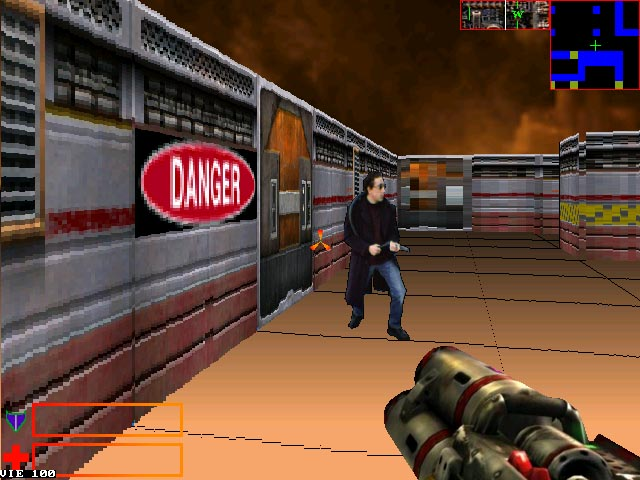
\includegraphics[height=5cm]{Allegroexample1}
\label{fig:allegro3d}}
\subfloat[Ejemplo 2D]{
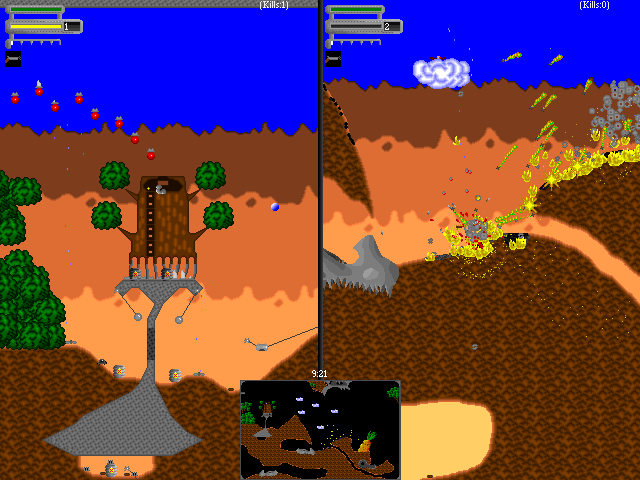
\includegraphics[height=5cm]{Allegroexample2}
\label{fig:allegro2d}}
\caption{Ejemplos de la potencia gráfica de la librería Allegro}
\end{figure}
%%%%%%%%%%%%%%%%%%%%%%%%%%%%%%%%%%%%%%%%%%%%%%%%%%%%%%%%%%%%%%

\section{Algoritmos de clustering}
El primer enfoque de nuestra aplicación fue basarnos en la densidad de objetos
en el espacio, con el objetivo de centrarnos en áreas con mayor densidad (y por 
tanto, mayor número de objetos a introducir en la CSU). Dado que nos interesa 
agrupar elementos en un espacio reducido, delimitado por el tamaño de la CSU,
prestaremos atención a los algoritmos de clustering.

Un algoritmo de agrupamiento (en inglés, clustering) es un procedimiento de 
agrupación de una serie de vectores de acuerdo con un criterio. Esos criterios
son por lo general distancia o similitud. La cercanía se define en términos de
una determinada función de distancia, como la euclídea, aunque existen otras más
robustas o que permiten extenderla a variables discretas. La medida más
utilizada para medir la similitud entre los casos es las matriz de correlación 
entre los n$\times$n casos. Sin embargo, también existen muchos algoritmos que
se basan en la maximización de una propiedad estadística llamada verosimilitud.

Generalmente, los vectores de un mismo grupo (o clústers) comparten propiedades
comunes. El conocimiento de los grupos puede permitir una descripción sintética
de un conjunto de datos multidimensional complejo. De ahí su uso en minería de 
datos. Esta descripción sintética se consigue sustituyendo la descripción de 
todos los elementos de un grupo por la de un representante característico del 
mismo.

Ninguno de los algoritmos clásicos de clustering cumple con las características
exactas de nuestro problema, por lo que se tuvo que investigar un poco como
funciona cada uno de ellos. Hay una gran diversidad de algoritmos, algunos muy
antiguos y otros bastante recientes, pero casi todos tienen en común la
dependencia de cierto tipo de parámetros condicionantes. Este tipo de
dependencia varía bastante el resultado, y no siempre resulta fácil saber qué se
está cambiando o cómo adecuarlo a nuestro problema. A continuación se muestran
algunos de los que se han analizado y estudiado con el fin de utilizarlos.

\subsection{K-means}

K-means \cite{Hartigan:1979:KMC} es un método de agrupamiento, que tiene como
objetivo la partición de un conjunto n en k grupos en el que cada observación
pertenece al grupo más cercano a la media. Esto da lugar a una 
compartimentación del espacio de datos en celdas de Voronoi.

El problema es computacionalmente difícil (NP-duro). Sin embargo, hay
heurísticas eficientes que se emplean comúnmente y convergen rápidamente a un
óptimo local. Estos suelen ser similares a los algoritmos de
esperanza-maximización de mezclas de distribuciones gausianas por medio de un
enfoque de refinamiento iterativo empleado por ambos algoritmos. Además, los dos
algoritmos usan los centros que los grupos utilizan para modelar los datos, sin
embargo k-means tiende a encontrar grupos de extensión espacial comparable,
mientras que el mecanismo esperanza-maximización permite que los grupos tengan
formas diferentes.

%%%%%%%%%%%%%%%%%%% Fig. %%%%%%%%%%%%%%%%%%%%%%%%%%%%%%%%%%%
\begin{figure}[!htb]
\centering
\subfloat[Entrada]{
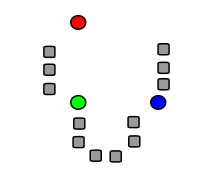
\includegraphics[height=2.5cm]{K_Means_Example_Step_1}
\label{fig:k_means1}}
\subfloat[Paso 1]{
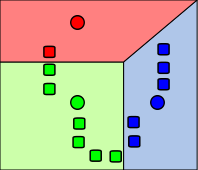
\includegraphics[height=2.5cm]{K_Means_Example_Step_2}
\label{fig:k_means2}}
\subfloat[Paso 2]{
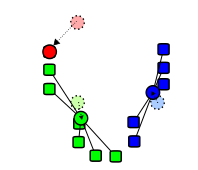
\includegraphics[height=2.5cm]{K_Means_Example_Step_3}
\label{fig:k_means3}}
\subfloat[Salida]{
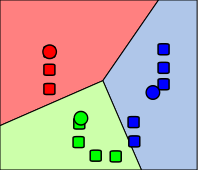
\includegraphics[height=2.5cm]{K_Means_Example_Step_4}
\label{fig:k_means4}}
\caption{Ejemplo de cómo funciona el K-means}
\end{figure}
%%%%%%%%%%%%%%%%%%%%%%%%%%%%%%%%%%%%%%%%%%%%%%%%%%%%%%%%%%%%%%

Como se trata de un algoritmo heurístico, no hay ninguna garantía de que
converja al óptimo global, y el resultado puede depender de los grupos
iniciales. Como el algoritmo suele ser muy rápido, es común para ejecutar
varias veces con diferentes condiciones de partida. Sin embargo, en el peor de
los casos, k-means puede ser muy lento para converger: en particular, se ha 
demostrado que existen conjuntos de determinados puntos, incluso en 2
dimensiones, en la que k-means toma tiempo exponencial.

\subsection{DBSCAN}

DBSCAN: Density-based spatial clustering of applications with noise (Agrupación
espacial basada en la densidad de aplicaciones con ruido) \cite{Ester:1996:SIC}, 
\cite{Wiki:2013:DBS} es un algoritmo de clustering de datos propuesto por Martin
Ester, Hans-Peter Kriegel, Jörg Sander y Xiaowei Xu en 1996. Se trata de un
algoritmo de clustering basado en la densidad, ya que encuentra un número de
clusters a partir de la distribución de la densidad estimada de nodos
correspondientes. DBSCAN es uno de los algoritmos de agrupamiento más común y
también el más citado en la literatura científica.

La definición de un conjunto en DBSCAN se basa en la noción de
accesibilidad-densidad. Básicamente, un punto $q$ es directamente accesible
desde un punto $p$ si no está más lejos que una distancia dada $\varepsilon$ (es 
decir, es parte de su $\varepsilon$-vecindad) y si $p$ está rodeado por
suficientes puntos de tal manera que uno pueda considerar $p$ y $q$ para ser
parte de un clúster. $q$ se denomina densidad alcanzable a partir de $p$ si hay
una secuencia de $p_1,\ldots,p_n$ de puntos con $p_1$ = p y $p_n$ = q donde cada 
$p_{i+1}$ es directamente accesible desde $p_i$.

Tenga en cuenta que la relación de la densidad alcanzable no es simétrica. $q$
podría estar al borde de un clúster, que tiene insuficiente cantidad de vecinos
a contar tan denso en sí. Esto detendría el proceso de encontrar una ruta que se 
detiene con el primer punto no denso. Por el contrario, empezar la ruta desde
$q$ podría encontrar un camino hasta $p$. Debido a esta asimetría, se introduce
la noción de densidad-conectada: dos puntos $p$ y $q$ están
densamente-conectados si hay un punto $o$ de tal manera que tanto $p$ como $q$
son la densidad alcanzable a partir de $o$. La densidad-conectada es simétrica.

Un clúster, que es un subconjunto de los puntos de la base de datos, satisface
dos propiedades:
\begin{itemize}
\item Todos los puntos dentro de la agrupación son mutuamente denso-conectados.
\item Si un punto está denso-conectado con cualquier punto de la agrupación, 
forma parte del grupo también.
\end{itemize}

DBSCAN requiere dos parámetros: $\varepsilon$ (EPS) y el número mínimo de puntos 
requeridos para formar un clúster (MinPts). Se inicia con un punto de partida 
arbitrario que no ha sido visitado. La $\varepsilon$-vecindad de este punto se 
recupera, y si contiene suficientes puntos, se inicia un clúster. De lo
contrario, el punto es considerado como ruido. Tenga en cuenta que este punto más 
adelante se podría encontrar en una $\varepsilon$-ambiente suficientemente
grande de un punto diferente y por lo tanto, formar parte de un clúster.

Si se encuentra un punto para ser una parte densa de un clúster, su 
$\varepsilon$-vecindad es también parte de ese grupo. Por lo tanto, se añaden
todos los puntos que se encuentran dentro de la $\varepsilon$-vecindad, así como
su propia $\varepsilon$-vecindad cuando también son densos. Este proceso
continúa hasta que el clúster  de densidad-conectada se halla por completo.
Entonces, un nuevo punto no visitado es recuperado y procesado, llevando al
descubrimiento de un clúster adicional o ruido.

%%%%%%%%%%%%%%%%%%%%% Fig. %%%%%%%%%%%%%%%%%%%%%%%%%%%%%%%%%%%
\begin{figure}[ht]
\centering
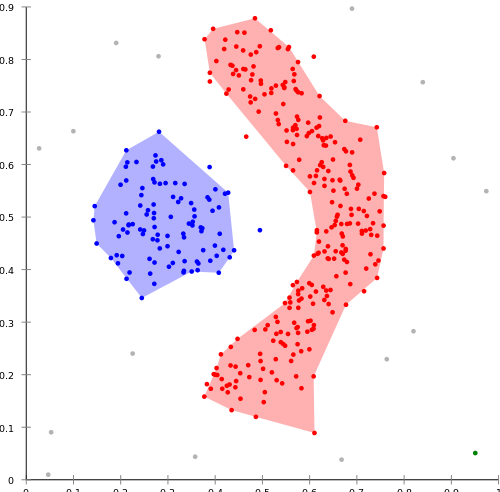
\includegraphics[height=10cm]{DBSCAN-density-data}
\label{fig:dbscan0}
\caption{Ejemplo del resultado del DBSCAN. Los puntos en gris son ruido}
\end{figure}
%%%%%%%%%%%%%%%%%%%%%%%%%%%%%%%%%%%%%%%%%%%%%%%%%%%%%%%%%%%%%

Ventajas
\begin{itemize}
\item DBSCAN no requiere especificar el número de grupos en los datos a priori,
como hace el k-means.
\item DBSCAN puede encontrar grupos de forma arbitraria. Se puede incluso
encontrar un clúster completamente rodeado por (pero no conectado a) un clúster
diferente. Debido al parámetro MinPts, el llamado efecto de enlace único
(diferentes grupos que se conectan por una delgada línea de puntos) se reduce.
\item DBSCAN tiene una noción de ruido.
\item DBSCAN requiere sólo dos parámetros y es insensible a la ordenación de los 
puntos en la base de datos. (Sin embargo, los puntos que se encuentren en el
borde de dos grupos diferentes pueden intercambiar pertenencia al clúster si se
cambia el orden de los puntos, y la asignación de clúster es único sólo hasta el
isomorfismo.)
\item DBSCAN está diseñado para su uso con bases de datos que pueden acelerar
las consultas de región, por ejemplo, mediante un árbol R*.
\end{itemize}

Desventajas
\begin{itemize}
\item La calidad de DBSCAN depende de la medida de distancia utilizado en la
función regionQuery(P,$\varepsilon$). La distancia métrica más común es la
distancia euclídea. Especialmente para los datos de grandes dimensiones, este 
indicador puede resultar casi inútil debido a la llamada ``maldición de la
dimensionalidad'', por lo que es difícil encontrar un valor adecuado para 
$\varepsilon$. Este efecto, sin embargo, también está presente en cualquier otro
algoritmo basado en la distancia euclídea. 
\item DBSCAN no puede agrupar conjuntos de datos correctamente si estos tienen
una gran diferencia en la densidad, ya que la combinación MinPts-$\varepsilon$
no puede entonces ser elegida adecuadamente para todos los grupos.
\end{itemize}

Todos estos algoritmos trabajan bastante bien cuando existen áreas más o menos 
diferenciadas unas de otras, sin embargo la mayoría de las ocasiones se trata
con datos dispersos de manera uniforme, con lo que el uso de estos algoritmos
puede ser más un inconveniente que una ventaja. Por otro lado, todos nuestros
objetos son relevantes, por lo que no podemos arriesgarnos a que se les tome por
ruido y, por lo tanto, se pierdan.

\section{Heurísticas}

En computación, dos objetivos fundamentales son encontrar algoritmos con buenos
tiempos de ejecución y buenas soluciones, usualmente las óptimas. Una heurística
es un algoritmo que abandona uno o ambos objetivos; por ejemplo, normalmente
encuentran buenas soluciones, aunque no hay pruebas de que la solución no pueda
ser arbitrariamente errónea en algunos casos; o se ejecuta razonablemente
rápido, aunque no existe tampoco prueba de que siempre será así. Las heurísticas
generalmente son usadas cuando no existe una solución óptima bajo las
restricciones dadas (tiempo, espacio, etc.), o cuando no existe del todo.

A menudo, pueden encontrarse instancias concretas del problema donde la
heurística producirá resultados muy malos o se ejecutará muy lentamente. Aun
así, estas instancias concretas pueden ser ignoradas porque no deberían ocurrir
nunca en la práctica por ser de origen teórico. Por tanto, el uso de heurísticas
es muy común en el mundo real.

A continuación se presenta la heurística que se ha evaluado, el método GRASP,
recomendada por el Doctor Marcos Moreno Vega.

\subsection{GRASP} \label{sec:grasp}

%http://catarina.udlap.mx/u_dl_a/tales/documentos/lii/hernandez_r_cm/capitulo3.pdf

La palabra GRASP proviene de las siglas de Greedy Randomized Adaptive Search
Procedures que se puede traducir como: Procedimientos de Búsqueda Voraces 
Aleatorizados y Adaptativos.

El método GRASP se introduce inicialmente por Feo y Resende en
\cite{Mladenovic:1997:VNS}. Es un procedimiento iterativo que consiste en: una
fase de construcción y una fase de búsqueda local. Se obtiene una solución
factible durante la fase de construcción aplicando un procedimiento voraz. 
En cada iteración del procedimiento voraz se agrega un nuevo elemento a la 
solución de acuerdo al valor de una función voraz. En lugar de escoger siempre
el mejor elemento candidato, se construye una lista con los mejores candidatos,
de donde se selecciona uno aleatoriamente. El término adaptativo se refiere al
hecho de que los beneficios asociados con cada elemento son actualizados en cada
iteración de la fase de construcción para reflejar los cambios producidos por 
selecciones previas. Una vez que se construye una solución utilizando un 
procedimiento voraz, se realiza un procedimiento de búsqueda local. 

En el Algoritmo \ref{algo:grasp1} se muestra el pseudocódigo de esta heurística
y en las Secciones \ref{subs:grasp1}, \ref{subs:grasp2} y \ref{subs:grasp3} se
explican los procedimientos que intervienen en el algoritmo.

\subsubsection{Algoritmo GRASP}
\begin{algorithm}[H]
\While {(criterio no satisfecho)} {

Construye una solución inicial usando el procedimiento voraz

Realiza una búsqueda local para mejorar la solución construida.

}
\caption{Pasos del \texttt{GRASP}}
\label{algo:grasp1}
\end{algorithm}

\subsubsection{Algoritmo de fase de construcción del GRASP.} \label{subs:grasp1}

Sea $f$ una función voraz, $\alpha$ es valor del parámetro para controlar la
aleatoriedad del procedimiento, $x$ una solución parcial, $C$ el conjunto de 
elementos candidato y $RCL$ la lista restringida de candidatos.

\begin{algorithm}[H]
$x \leftarrow {\O}$

Inicializa el conjunto de candidatos $C$

\While{$x$ infactible} {

  $a = min\{f(t), t \in C\}$

  $b = max\{f(t), t \in C\}$

  $RCL = \{c \in C, f(c)\le a + \alpha(b - a)\}$

  Seleccionar aleatoriamente un elemento $c \in RCL$

  $x \leftarrow x \cup\{c\}$

  Actualizar $C$
}

\caption{Pseudo-código constructivo para \texttt{GRASP}}
\label{algo:grasp2}
\end{algorithm}

\subsubsection{Algoritmo de búsqueda local.} \label{subs:grasp2}

Sea $f(x)$ la función a minimizar, $x$ una solución factible y $N(x)$ una
estructura de vecindad.

\begin{algorithm}[H]
$CriterioParada \leftarrow$ falso

\While{no se satisfaga $CriterioParada$} {

$x' = arg min\{f(y): y \in N(x)\}$

\eIf{$(f(x') < f(x))$} {$x \leftarrow x'$} {$CriterioParada \leftarrow$ cierto}
}
\caption{Pseudo-código de la búsqueda local}
\label{algo:grasp3}
\end{algorithm}
\subsubsection{Algoritmo voraz.} \label{subs:grasp3}

Sean $S$ una solución parcial, $E$ el conjunto factible de elementos que pueden 
ser añadidos a la solución parcial, $e_i·$ los elementos del conjunto $E$ y $g$
una función voraz. 

\begin{algorithm}[H]
$S \leftarrow \O$

  \While{$S$ no factible} {
  Evaluar la función voraz $g$ para cada elemento de E
  
	Seleccionar el mejor elemento $e \in E$ de acuerdo con el valor de la función voraz $g$
  
	$S \leftarrow S\cup\{e\}$
  
	Actualizar $E$
}
\caption{Método voraz para seleccionar los mejores elementos de la búsqueda}
\label{algo:grasp4}
\end{algorithm}

El objetivo de utilizar este método es mejorar la solución inicial obtenida con
nuestro algoritmo constructivo. Se explicará este proceso y hasta qué punto se ha
utilizado dentro de \CSUO{} en el Capítulo \ref{chap:aplication}.
